Оптимальное распределение ресурсов в аналитических постановках изучается с помощью дизайна механизмов.
Современный подход был предложен и развит Леонидом Гурвичем \cite{hurwicz1960optimality}.
В его работе изучается проблемы доказательная эффективность организации рабочих процессов.

Механизм позволяет ограничить свободу действий игроков в системе таким образом, 
что действия агентов в доминантных стратегиях будут соответствовать ожиданиям принципала.

Строгое определение вводится через понятие байесовых игр с неполной информацией, 
предполагающих наличие нескольких многошаговых игр, направленных на формирование оптимальной стратегии. 


\begin{figure}[h]
    \centering
    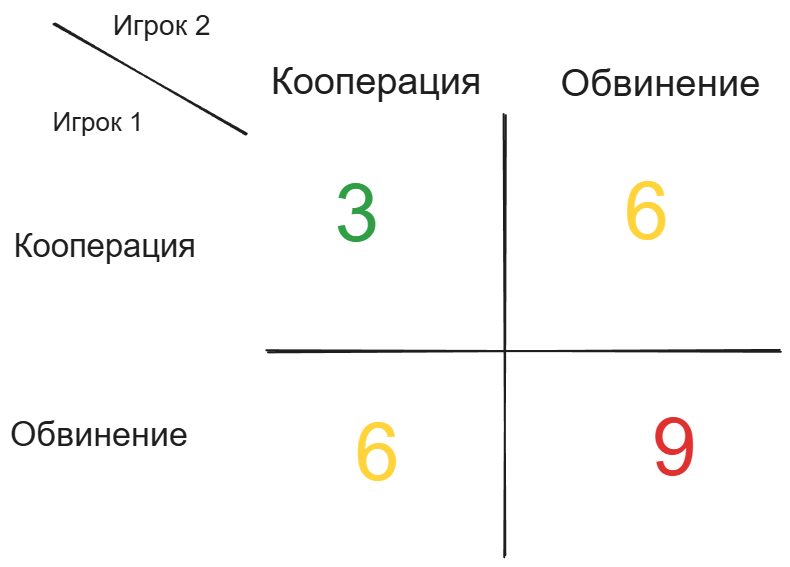
\includegraphics[width=0.5\textwidth]{assets/pedagogic/social/dilemma.excalidraw.png}
    \caption{Дилемма заключенного}
    \label{dilemma}
\end{figure}


\textit{Определение} \textbf{Байесова игра} это набор исходов $(N,O,\Theta)$ таких что,
\begin{itemize}
    \item $\mathbf{N}$ конечное множество агентов $n$
    \item $O$ множество исходов
    \item  $\Theta = \Theta_1 \times \Theta_2 \dots \Theta_n $ множество 
    \item $u = (u_1, \dots, u_N)$, где $u_i: O \times \Theta \rightarrow \mathrm{R}$  функция полезности для игрока $i$
\end{itemize}

\textit{Определение} \textbf{Механизм} для байесовой игры это пара $(A,M)$, где \begin{itemize}
    \item $A = A_1 \times \dots \times A_n$ набор действий доступный агенту $i$
    \item $M: A \rightarrow \Pi(O)$ соединяет действия с распределением возможностей
\end{itemize}

Изучение механизма заключается в анализе доминантных стратегий и равновесных состояний, к которым они приводят. 


\textit{Определение} В заданной байесовой игре, механизм является \textbf{воплощением доминантной стартегии} 
социального выбора функции $C$, если для любого вектора полезности $u$ , 
у игры есть равновесие в доминантной стратегии, и для любого равновесия $a^*$ выполняется $M(a^*) = C(u)$


Теория механизмов используется В
постановках с ассиметричной информацией
и достаточно большим числом игроков, что
как правило не позволяет наивно перебрать возможные исходы.


Предполагается, что функция пользы
от единицы объекта задается 
функцией распределения $F$,
ограниченной на промежутке $\left[0,
hat{v}\right]$. Обозначим квантиль распределения 
как $q(v_i) = 1 - F(v_i) \in \left[0,1\right]$.

Тогда функция полезности при заданном векторе ставок 
$\mathbf{b} = \left(b_1, \dots, b_n\right)$
задается как 
$$
    u_i(\mathbf{b};q_i) = v(q_i) \cdot x_i(\mathbf{b})
$$




